\section{Projection-based reduction of contact}\label{sec:vf-bal}

\subsection*{Concept and purpose}

\citet{balajewicz2016contact} reduce Lagrange-multiplier contact by Galerkin projection with two bases of the same size: an SVD basis for the displacements, and a \emph{non-negative} basis for the contact forces, obtained by non-negative matrix factorisation (NMF), so that the reduced multipliers stay non-negative by construction. A greedy sampler chooses the training parameters with a contact-condition indicator that needs no linear solve. Three experiments test the method: a static membrane against a parametrised obstacle, its dynamic version, and two clamped plates in dynamic contact; the last also tests how far the temporal snapshots can be down-sampled. It is the method of Chapter~\ref{ch:hyper}, and the study checks what the packages already contain of it and what had to be added.

\subsection*{Mathematics as implemented}

The semi-discrete contact problem is $\mathbf M\ddot{\mathbf u}+\mathbf K\mathbf u=\mathbf f+\mathbf B^{T}\boldsymbol\lambda$, $\mathbf B\mathbf u-\mathbf c\ge\mathbf 0$, $\boldsymbol\lambda\ge\mathbf 0$, $\boldsymbol\lambda^{T}(\mathbf B\mathbf u-\mathbf c)=0$. After implicit time discretisation each step is the saddle-point problem
\begin{equation}\label{eq:bl-sp}
\min_{\mathbf v}\max_{\boldsymbol\mu\ge\mathbf 0}\ \tfrac12\mathbf v^{T}\mathbf A\mathbf v-\mathbf v^{T}\mathbf b-\boldsymbol\mu^{T}(\mathbf B\mathbf v-\mathbf c).
\end{equation}
With $\mathbf u\approx\mathbf U\mathbf u_r$ and $\boldsymbol\lambda\approx\mathbf U_\lambda\boldsymbol\lambda_r$, $\mathbf U_\lambda\ge\mathbf 0$, the reduced matrices are
\begin{equation}\label{eq:bl-red}
\mathbf A_r=\mathbf U^{T}\mathbf A\mathbf U,\qquad\mathbf B_r=\mathbf U_\lambda^{T}\mathbf B\mathbf U,\qquad\mathbf c_r=\mathbf U_\lambda^{T}\mathbf c,
\end{equation}
and the reduced multipliers $\boldsymbol\lambda_r\ge\mathbf 0$ give $\mathbf U_\lambda\boldsymbol\lambda_r\ge\mathbf 0$ automatically. The displacement basis $\mathbf U$ is a POD of the snapshots; the dual basis is the NMF of the multiplier snapshots,
\begin{equation}\label{eq:bl-nmf}
\mathbf X_\lambda\approx\mathbf U_\lambda\mathbf V_\lambda,\qquad\mathbf U_\lambda,\mathbf V_\lambda\ge\mathbf 0,
\end{equation}
computed by hierarchical alternating least squares with a non-negative SVD start (\anchor{rom_engine.nonneg_dual_basis}); contact-free (zero) dual snapshots are dropped.

\emph{Greedy sampling.} The next parameter is the candidate with the largest indicator
\begin{equation}\label{eq:bl-ind}
I=\sum_n\alpha_1\phi(\mathbf r_1)^2+\alpha_2\lVert\mathbf r_2\rVert^2+\alpha_3\phi(\mathbf r_3)^2,
\end{equation}
with the penetration $\mathbf r_1=\mathbf B\mathbf u-\mathbf c$, the complementarity $\mathbf r_2=\mathbf B^{+}(\mathbf A\mathbf u-\mathbf b)\odot(\mathbf B\mathbf u-\mathbf c)$, the force sign $\mathbf r_3=\mathbf B^{+}(\mathbf A\mathbf u-\mathbf b)$ and $\phi(\mathbf v)=\lVert[\mathbf v]_-\rVert$. No linear solve is needed. The error measures are squared relative norms in per cent (the publication's Eqs.~16--17), implemented literally.

\subsection*{What the packages provided}

\Cref{tab:vf-bl-cap} is the capability assessment made before the runs. The reduced-order side of the publication is implemented in \rom{} (\texttt{nonneg\_dual\_basis}, \texttt{ContactROM}, \texttt{solve\_reduced\_contact}, \texttt{contact\_condition\_indicator}, \texttt{greedy\_contact\_sampling}); the finite element side is adequate for plates and for complementarity-based contact up to a few thousand constraints, and four things were bridged with local code, each cross-checked against the package where they overlap.

\begin{table}[tbp]
\centering\footnotesize
\caption{Paper ingredient, package support and what was done.}\label{tab:vf-bl-cap}
\begin{tabularx}{\linewidth}{@{}>{\raggedright\arraybackslash}p{3.3cm} >{\raggedright\arraybackslash}p{3.2cm} >{\raggedright\arraybackslash}X@{}}
\toprule
Ingredient & Package support & Evidence or action\\
\midrule
Q4 scalar membrane (Laplace) element & missing in \fea{} & assembled locally (9-point stencil, lumped mass); free-membrane centre value $-0.7382$ against analytic $\approx-0.737$\\
Mindlin / Kirchhoff plate & Mindlin only & Mindlin used; clamped-plate centre deflection within $0.3\,\%$ of the analytic $0.00126\,qL^4/D$, first frequency within $0.4\,\%$ (24$\times$24 mesh)\\
Static contact solver & yes, dense (forms $\mathbf B\mathbf K^{-1}\mathbf B^{T}$) & fine to about 3k constraints, impossible at 39\,601 ($\approx12.5$ GB); a sparse primal--dual active-set solver was written and agrees with the package active-set, Lemke and projected-Gauss--Seidel solvers to $10^{-15}$ (check C1)\\
Dynamic contact solver & first-order two-step scheme only & free-vibration test: package scheme error $4.7\times10^{-2}$ at $\Delta t=2.5\times10^{-3}$ (order 1), local BDF2 $7.8\times10^{-4}$ (order 2) (C4); BDF2 contact stepping written locally\\
POD, SVD basis & yes & ---\\
NMF dual basis & yes & non-negative by construction (minimum entry $\ge10^{-17}$); fit within $1\,\%$ of SVD at rank 8 (C5)\\
Reduced contact solve & yes (static \texttt{ContactROM}, \texttt{solve\_reduced\_contact}) & full bases reproduce the full model to $2\times10^{-15}$ (C2); the reduced dynamic loop was written locally\\
Error indicator & yes & matches the vectorised formula exactly (C3: $0.77469$ both); the $\alpha_2,\alpha_3$ terms use a dense least-squares per call and do not scale, $\alpha=(1,0,0)$ is matrix-free\\
Greedy loop & yes & reproduced an independent implementation's selection sequence exactly (static, 20 iterations); trajectory snapshots, the $p(N_{\rm iter})$ growth schedule and the relative stopping test are not provided\\
\bottomrule
\end{tabularx}
\end{table}

The building-block checks are in \Cref{tab:vf-bl-checks}.

\begin{table}[tbp]
\centering\footnotesize
\caption{Building-block checks C1--C6.}\label{tab:vf-bl-checks}
\begin{tabularx}{\linewidth}{@{}>{\raggedright\arraybackslash}p{4.8cm} >{\raggedright\arraybackslash}X@{}}
\toprule
Check & Result\\
\midrule
C1 sparse PDAS against package active-set / Lemke / PGS (529-dof obstacle) & max difference $1.1\times10^{-15}$ / $7.8\times10^{-16}$ / $7.8\times10^{-16}$\\
C2 \texttt{ContactROM} with $\mathbf U=\mathbf U_\lambda=\mathbf I$ against full & $1.7\times10^{-15}$ ($u$), $2.1\times10^{-15}$ ($\lambda$)\\
C3 package indicator against local, $\alpha=(1,1,1)$ & $0.7746922$ against $0.7746922$\\
C4 free-membrane error at $t=2$ ($\Delta t=10^{-2}$, $5\times10^{-3}$, $2.5\times10^{-3}$) & BDF2 $1.2\times10^{-2}$, $3.1\times10^{-3}$, $7.8\times10^{-4}$ (order 2); package two-step $1.6\times10^{-1}$, $8.7\times10^{-2}$, $4.7\times10^{-2}$ (order 1)\\
C5 NMF against SVD relative fit, rank 4 / 8 / 16 & $0.385$ / $0.0249$ / $1.4\times10^{-9}$ against $0.377$ / $0.0247$ / $5.7\times10^{-16}$; the SVD basis has minimum entry $-0.97$ to $-1.0$, NMF $\ge0$\\
C6 reduced complementarity solve, $p=20/40/100/200$ & 1.0 / 1.4 / 1.9 / 8.0 ms\\
\bottomrule
\end{tabularx}
\end{table}

\subsection*{Geometry and mesh}

\emph{Static and dynamic membrane.} A membrane on the unit square, $200\times200$ bilinear elements (39\,601 degrees of freedom) in the static case and $40\times40$ (1521) in the dynamic case, loaded by a uniform load $-10$ ($-\nabla^2u=f$, so the membrane deflects downward as in the publication's figure) and held up by an obstacle of two Gaussian bumps whose position $\gamma_1$ and height $\gamma_2$ are the parameters, $\gamma\in[0.3,0.6]\times[0.2,0.6]$ (\Cref{fig:vf-bl-obstacle}). \emph{Two plates.} Two identical clamped steel plates ($L=1$~m, $h=1$~mm, $\rho=7800$, $E=200$~GPa, $\nu=0.3$) with a $4$~cm gap, each meshed with $24\times24$ Mindlin elements, 3174 degrees of freedom and 529 gap constraints at facing nodes (the publication's plates are Kirchhoff plates with one degree of freedom per node and 20\,000 in all); a pressure pulse acts only on the lower plate (\Cref{fig:vf-bl-two}). \Cref{tab:vf-bl-setup} lists the settings.

\begin{figure}[tbp]
\centering
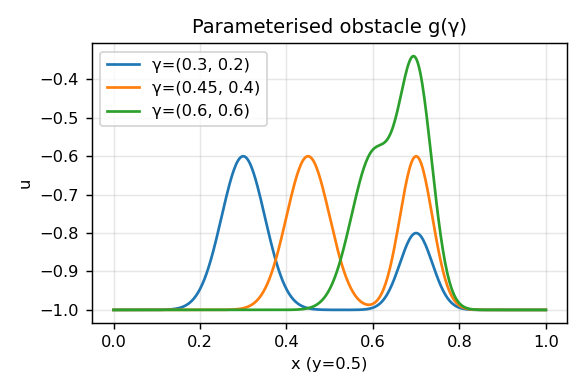
\includegraphics[width=0.7\linewidth]{figures/ch14r/bl_obstacle.png}
\caption{Obstacle of the membrane problem and its parametrisation. Plot of the reproduction report.}\label{fig:vf-bl-obstacle}
\end{figure}

\begin{figure}[tbp]
\centering
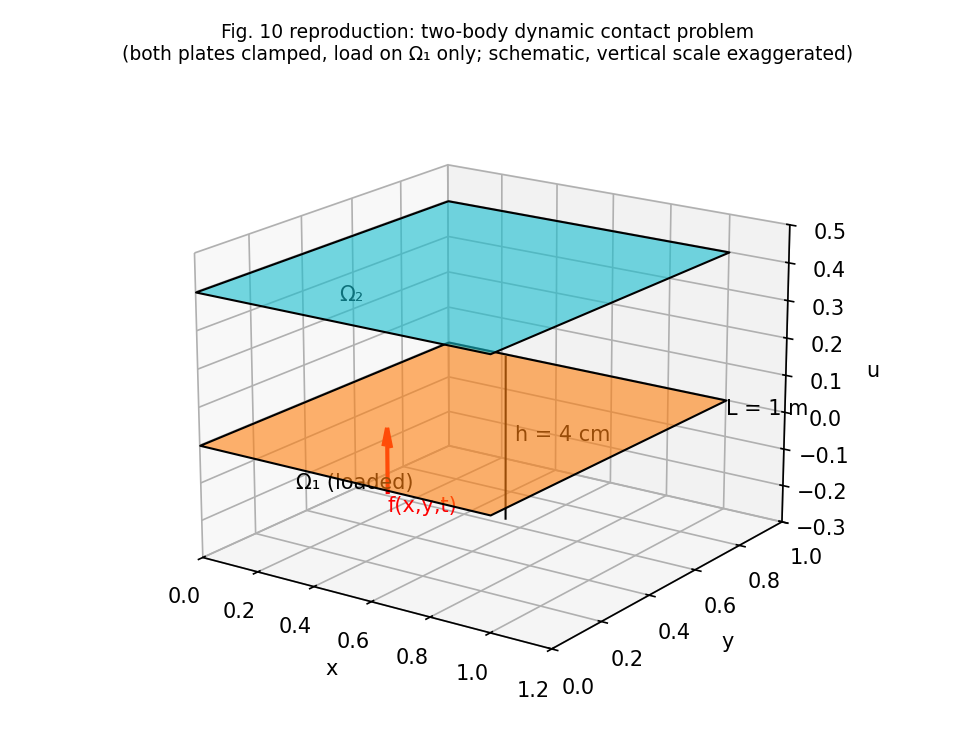
\includegraphics[width=0.6\linewidth]{figures/ch14r/bl_two.png}
\caption{Two-body set-up: two clamped plates with a 4~cm gap and a pressure pulse on the lower plate; the non-penetration constraint is imposed at every pair of facing nodes (529). Redrawn schematic, vertical scale exaggerated; not simulation output. Plot of the reproduction report.}\label{fig:vf-bl-two}
\end{figure}

\begin{table}[tbp]
\centering\footnotesize
\caption{Set-up of the three experiments.}\label{tab:vf-bl-setup}
\begin{tabularx}{\linewidth}{@{}>{\raggedright\arraybackslash}p{2.6cm} >{\raggedright\arraybackslash}X >{\raggedright\arraybackslash}X >{\raggedright\arraybackslash}X@{}}
\toprule
 & Static obstacle & Dynamic obstacle & Two plates\\
\midrule
Size, this work (publication) & 39\,601 (40\,000) dofs & 1521 (40\,000) dofs & 3174 (20\,000) dofs\\
Time stepping & --- & BDF2 (BDF1 first step), $\Delta t=0.005$, 400 steps & BDF2, $\Delta t=2\times10^{-4}$, 2000 steps\\
Parameters & $\gamma\in[0.3,0.6]\times[0.2,0.6]$, $10\times10$ candidates & same range & non-parametric (reproduction mode, one parameter)\\
Greedy & 20 iterations, $p=p_\lambda=N_{\rm iter}$, first sample candidate 0 & 10 iterations, $p=p_\lambda=\lfloor2+(N_{\rm iter}-1)\,98/9\rfloor$ (2 to 100) & $p=p_\lambda=40$, all 2001 steps\\
Bases & snapshots used directly & SVD primal, NMF dual (150 HALS iterations) on active columns & as dynamic\\
Reference for errors & Eq.~16 on the 100 candidates; random sampling: 50 Latin hypercube draws of 20 samples & Eq.~17 over all time steps & Eq.~17 on $w$\\
\bottomrule
\end{tabularx}
\end{table}

\subsection*{Results: static obstacle (paper Figs.~3--5, full size)}

\Cref{tab:vf-bl-static} and \Cref{fig:vf-bl-static} give the greedy convergence. After 20 greedy samples the maximum error with $\alpha=(1,0,0)$ is $5.0\times10^{-4}\,\%$, a factor of 124 below the median of random sampling (median $6.3\times10^{-2}\,\%$, minimum $2.0\times10^{-2}$, maximum $0.22$), and the greedy loop with 10 samples ($4.4\times10^{-2}\,\%$) already beats the median of 20 random samples, as the publication states. The three indicator weightings $\alpha=(1,1,1)$, $(1,1,0)$, $(1,0,0)$ gave the \emph{identical} selection sequence ($0$, $99$, $64$, $92$, $44$, $80$, \dots) and errors, so the publication's difference between them was not reproduced; the oracle greedy on the true error is worse than the indicator-driven one from $N_{\rm iter}\ge13$ ($1.7\times10^{-3}\,\%$ against $5.0\times10^{-4}\,\%$ at 20), because greedy on the maximum error is myopic; and the package's \texttt{greedy\_contact\_sampling} gave the identical 20-element sequence as the local loop.

\begin{table}[tbp]
\centering\footnotesize
\caption{Static obstacle, $N_{\rm iter}=20$.}\label{tab:vf-bl-static}
\begin{tabular}{@{}lrr@{}}
\toprule
Quantity & Publication & This work\\
\midrule
Max relative error, greedy $\alpha=(1,0,0)$ & ``an order of magnitude'' below random $p=20$ & $5.0\times10^{-4}\,\%$ against random median $6.3\times10^{-2}\,\%$ ($124\times$ lower)\\
Greedy at $p\approx10$ against random $p=20$ & equal accuracy & $4.4\times10^{-2}\,\%<6.3\times10^{-2}\,\%$\\
Mean relative error, greedy 20 & --- & $3.6\times10^{-5}\,\%$ (random median $6.5\times10^{-3}\,\%$)\\
Indicator weights & $\alpha_1$ only is best & identical sequences\\
Oracle on the true error & lowest curve & worse at $N_{\rm iter}\ge13$\\
\bottomrule
\end{tabular}
\end{table}

\begin{figure}[tbp]
\centering
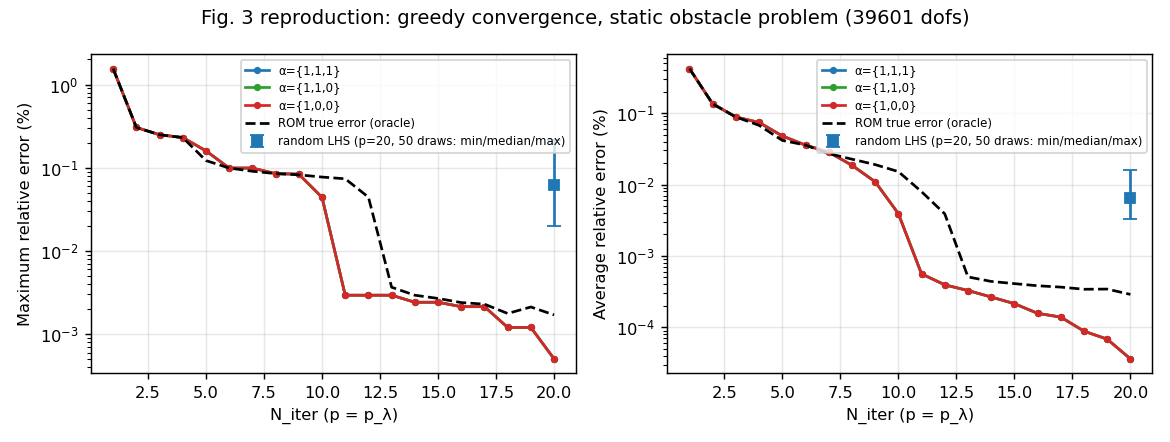
\includegraphics[width=0.9\linewidth]{figures/ch14r/bl_static.png}
\caption{Static obstacle, greedy convergence against random sampling for the indicator weightings and the oracle. Plot of the reproduction report.}\label{fig:vf-bl-static}
\end{figure}

\begin{figure}[tbp]
\centering
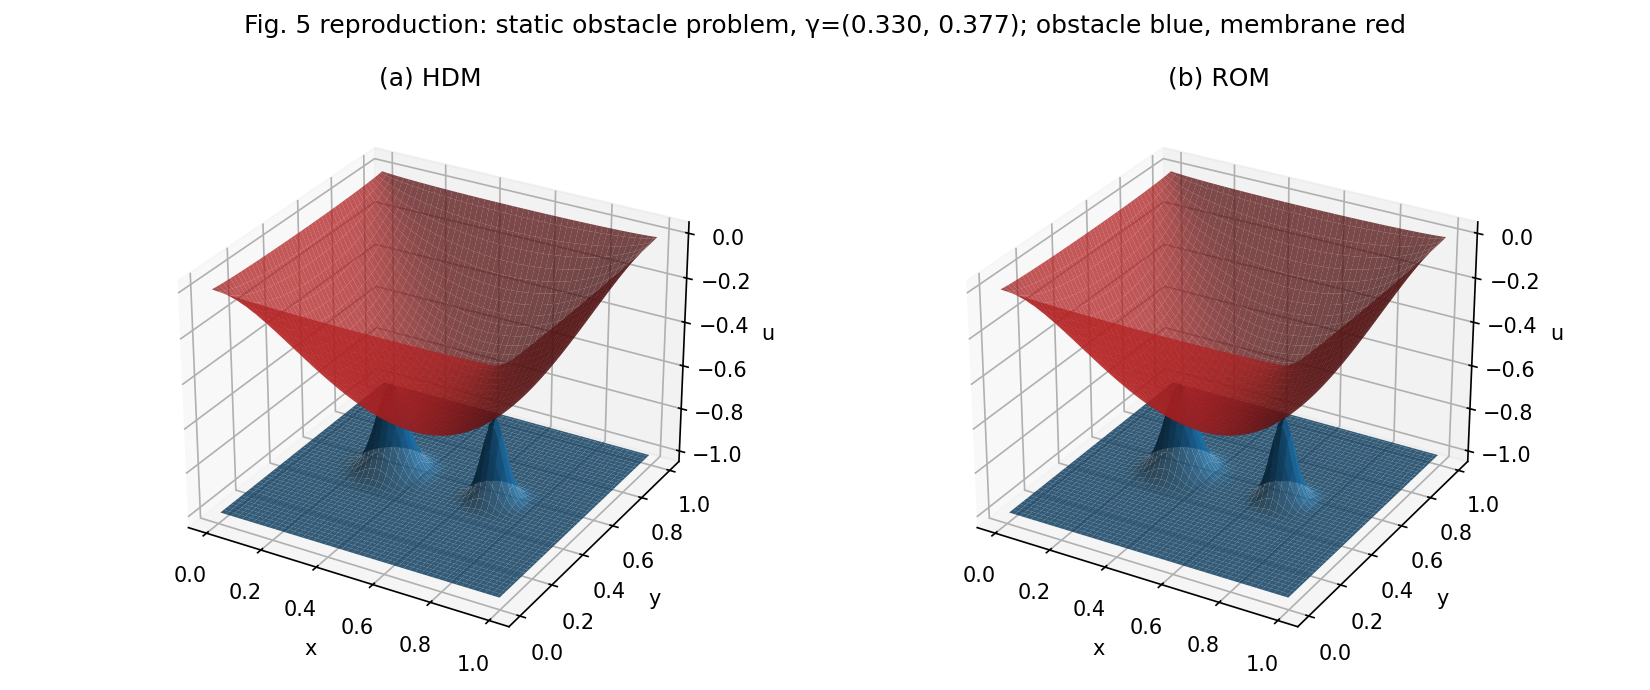
\includegraphics[width=0.9\linewidth]{figures/ch14r/bl_static3d.png}
\caption{Static solution: the membrane (red) sags under the load and is held by the two bump tips of the obstacle (blue), left bump at $x=\gamma_1=0.33$ and right bump at $x=0.7$ with height $\gamma_2$. The ROM built from 20 greedy snapshots ($p=p_\lambda=20$, 39\,601-dof full model) is visually indistinguishable from the full model. Plot of the reproduction report.}\label{fig:vf-bl-static3d}
\end{figure}

At the publication's worst parameter $\gamma=(0.330,0.377)$ (off the grid) the displacement error is $1.5\times10^{-5}\,\%$, but the contact-force error is $52\,\%$ with an active-set overlap of $0.69$: displacement accuracy hides a poorer multiplier, which the publication does not report. Positivity over the 100 candidates ($p=p_\lambda=20$): the NMF dual basis gives minimum multiplier $0$ and worst full-space penetration $-1.3\times10^{-2}$ (only the projected constraint $\mathbf U_\lambda^{T}(\mathbf B\mathbf u-\mathbf c)\ge0$ is enforced); an SVD dual basis (not in the publication for the static case) gives minimum multiplier $-0.108$, penetration $-0.148$ and a maximum error of $4.0\,\%$ (mean $2.3\,\%$), about four orders worse.

\subsection*{Results: dynamic obstacle (paper Figs.~6--9)}

On the $40\times40$ mesh the error falls by a factor of 127 to 288 over ten greedy iterations for all indicator weightings (\Cref{tab:vf-bl-dyn}, \Cref{fig:vf-bl-dyn}), the publication's ``more than $100\times$ after 10 iterations, all strategies equal''; a candidate sweep of the final $\alpha=(1,0,0)$ ROM gives maximum $0.145\,\%$ and mean $0.070\,\%$.

\begin{table}[tbp]
\centering\footnotesize
\caption{Dynamic obstacle: maximum relative error (Eq.~17, \%) by iteration.}\label{tab:vf-bl-dyn}
\begin{tabular}{@{}lrrrrr@{}}
\toprule
Weights & $N_{\rm iter}=1$ & 2 & 5 & 10 & Reduction 1$\to$10\\
\midrule
$\alpha=(1,1,1)$ & 41.8 & 4.41 & 0.805 & 0.153 & 273$\times$\\
$\alpha=(1,1,0)$ & 41.8 & 10.9 & 0.808 & 0.329 & 127$\times$\\
$\alpha=(1,0,0)$ & 41.8 & 10.9 & 0.711 & 0.145 & 288$\times$\\
Oracle (true error) & 41.8 & 6.03 & 0.745 & 0.300 & 139$\times$\\
\bottomrule
\end{tabular}
\end{table}

\begin{figure}[tbp]
\centering
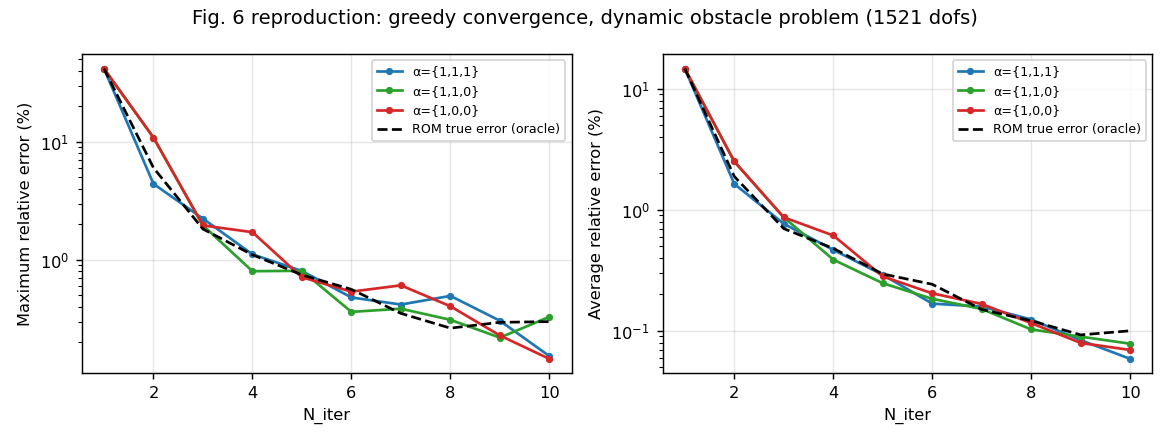
\includegraphics[width=0.9\linewidth]{figures/ch14r/bl_dyn.png}
\caption{Dynamic obstacle, greedy convergence. Plot of the reproduction report.}\label{fig:vf-bl-dyn}
\end{figure}

\begin{figure}[tbp]
\centering
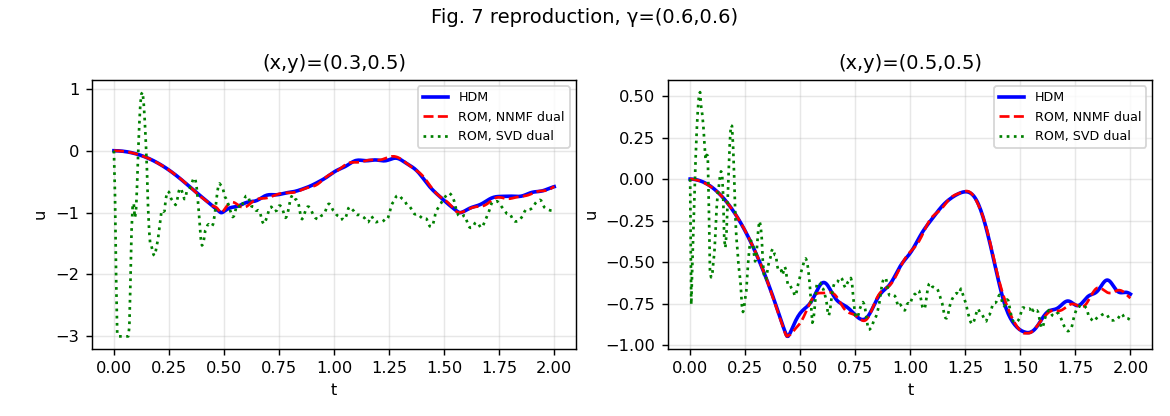
\includegraphics[width=0.95\linewidth]{figures/ch14r/bl_hist.png}
\caption{Time history of the final ROM ($p=p_\lambda=100$) at the off-training test parameter $\gamma=(0.6,0.6)$. Plot of the reproduction report.}\label{fig:vf-bl-hist}
\end{figure}

\Cref{tab:vf-bl-nmf} gives the publication's central qualitative claim at two test parameters: the SVD-dual ROM fails because positivity is lost (errors of about $300\,\%$, negative multipliers down to $-714$, penetrations more than 15 times the membrane depth), while the NMF-dual ROM tracks the full model. The field at $t=0.2$ for the worst-case test parameter is reproduced in shape and contact region (error $0.058\,\%$, \Cref{fig:vf-bl-dyn3d}).

\begin{table}[tbp]
\centering\footnotesize
\caption{NMF against SVD dual basis, dynamic obstacle.}\label{tab:vf-bl-nmf}
\begin{tabular}{@{}lrrr@{}}
\toprule
Test $\gamma$ & NMF dual: error / min $\lambda$ / min gap & SVD dual: error / min $\lambda$ / min gap\\
\midrule
$(0.6,0.6)$ & $0.083\,\%$ / 0 / $-1.5\times10^{-2}$ & $307\,\%$ / $-664$ / $-15.5$\\
$(0.300,0.288)$ & $0.058\,\%$ / 0 / $-1.3\times10^{-2}$ & $296\,\%$ / $-714$ / $-17.6$\\
\bottomrule
\end{tabular}
\end{table}

\begin{figure}[tbp]
\centering
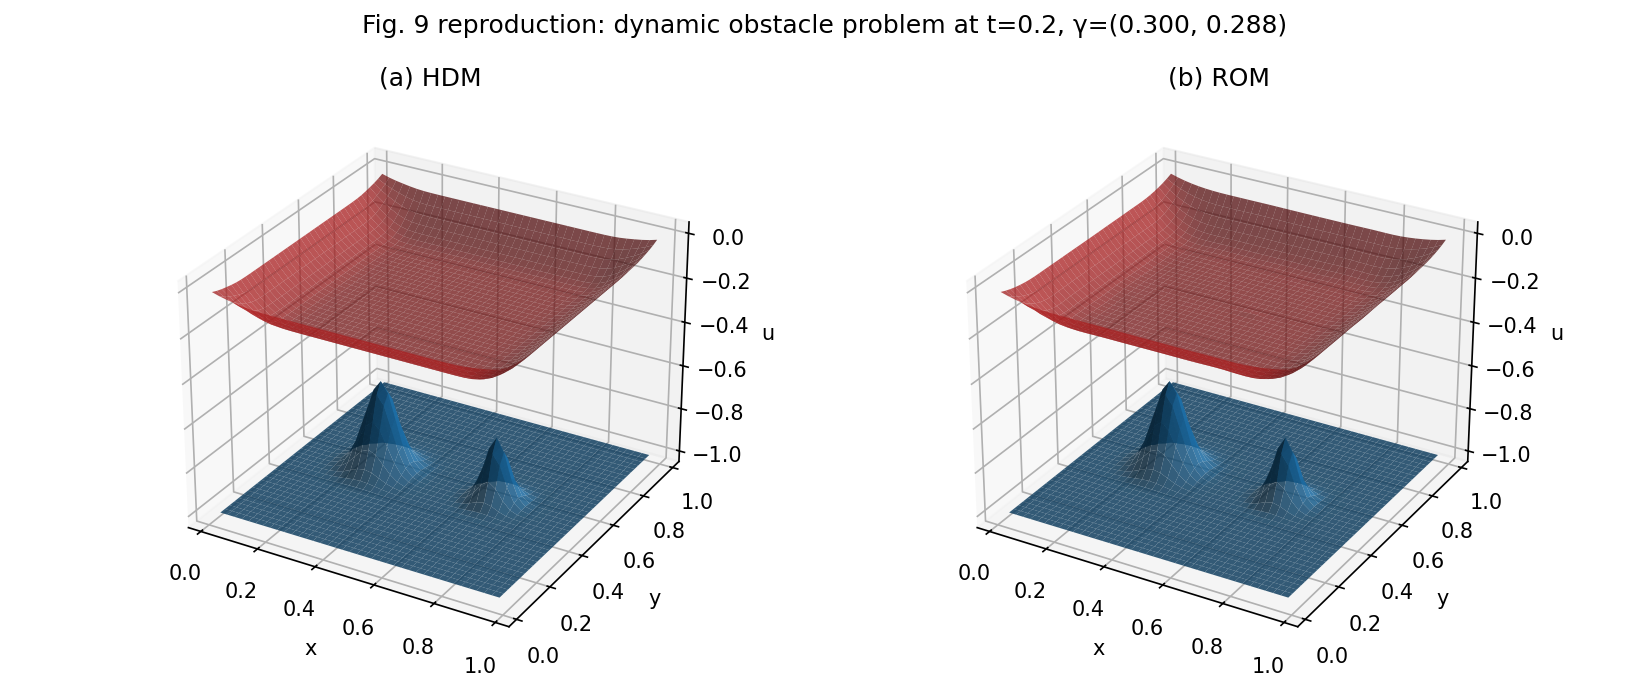
\includegraphics[width=0.9\linewidth]{figures/ch14r/bl_dyn3d.png}
\caption{Dynamic obstacle at $t=0.2$, $\gamma=(0.300,0.288)$: the 1521-dof full model against the NMF-dual ROM ($p=p_\lambda=100$); the membrane is still moving. Plot of the reproduction report.}\label{fig:vf-bl-dyn3d}
\end{figure}

\begin{figure}[tbp]
\centering
\includegraphics[width=1.0\linewidth]{figures/ch14_bal.pdf}
\caption{Dynamic obstacle problem of \citet{balajewicz2016contact} (1\,521 dofs). (a) Maximum error against the greedy iteration for the three indicator weightings and the true-error oracle (a reduction of \cvfBalRed{} for $\alpha=(1,0,0)$). (b), (c) Response at a test parameter: the NMF dual basis follows the full-order model (error \cvfBalNmf), the SVD dual basis does not (error \cvfBalSvd). Measured speed-up \cvfBalSpeed. Redrawn by \texttt{scripts/ch14\_assets.py} from the saved outputs of the study; the study itself was not re-run for this book.}\label{fig:vf-bal}
\end{figure}

\subsection*{Results: two-body dynamic contact (paper Figs.~10--13)}

Contact is active in 366 of the 2000 steps; the plate-centre amplitude is $0.126$~m (the publication's axis spans $\pm0.2$~m) and the peak contact force is $1.7\times10^3$~N per node (\Cref{fig:vf-bl-twohist}). \Cref{tab:vf-bl-two} gives the ROMs against a full-order run of $10.0$~s: the NMF dual with $p=p_\lambda=40$ (the publication's choice) has an error of $1.36\,\%$ and runs $13.5$ times faster, while the SVD dual of the same size fails ($41\,\%$, minimum multiplier $-2.9\times10^6$). At the single instant $t=0.4$~s the full-state field error of the $p=40$ ROM is $25\,\%$ (all degrees of freedom including rotations), far larger than the $1.4\,\%$ time-integrated error on $w$; the 3D snapshot looks close but is the harder test (\Cref{fig:vf-bl-two3d}).

\begin{table}[tbp]
\centering\footnotesize
\caption{Two plates: error (Eq.~17 on $w$), minimum multiplier, minimum gap and online time against the full model (10.0~s).}\label{tab:vf-bl-two}
\begin{tabular}{@{}lrrrr@{}}
\toprule
ROM & Error & Min $\lambda$ & Min gap (m) & Online time\\
\midrule
NMF dual, $p=p_\lambda=20$ & $1.84\,\%$ & 0 & $-6.7\times10^{-3}$ & 0.41 s (24.7$\times$)\\
\textbf{NMF dual, $p=p_\lambda=40$} & $\mathbf{1.36\,\%}$ & 0 & $-1.2\times10^{-2}$ & 0.74 s (13.5$\times$)\\
NMF dual, $p=p_\lambda=100$ & $0.040\,\%$ & 0 & $-1.7\times10^{-3}$ & 1.59 s (6.3$\times$)\\
SVD dual, $p=p_\lambda=40$ & $41\,\%$ & $-2.9\times10^{6}$ & $-0.50$ & 4.8 s (2.1$\times$)\\
\bottomrule
\end{tabular}
\end{table}

\begin{figure}[tbp]
\centering
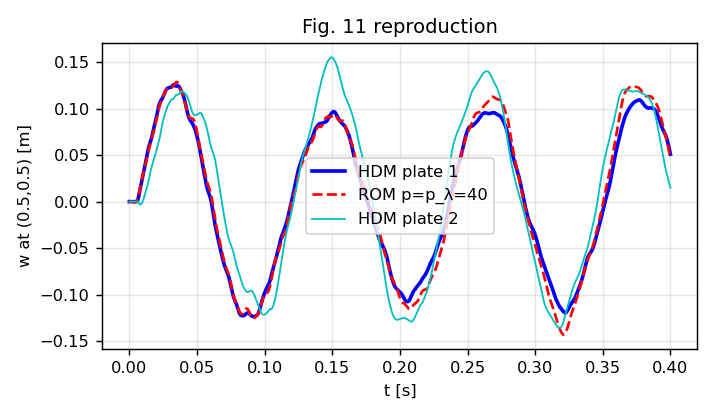
\includegraphics[width=0.95\linewidth]{figures/ch14r/bl_twohist.png}
\caption{Two plates: plate-centre time histories of the full model and the reduced models. Plot of the reproduction report.}\label{fig:vf-bl-twohist}
\end{figure}

\begin{figure}[tbp]
\centering
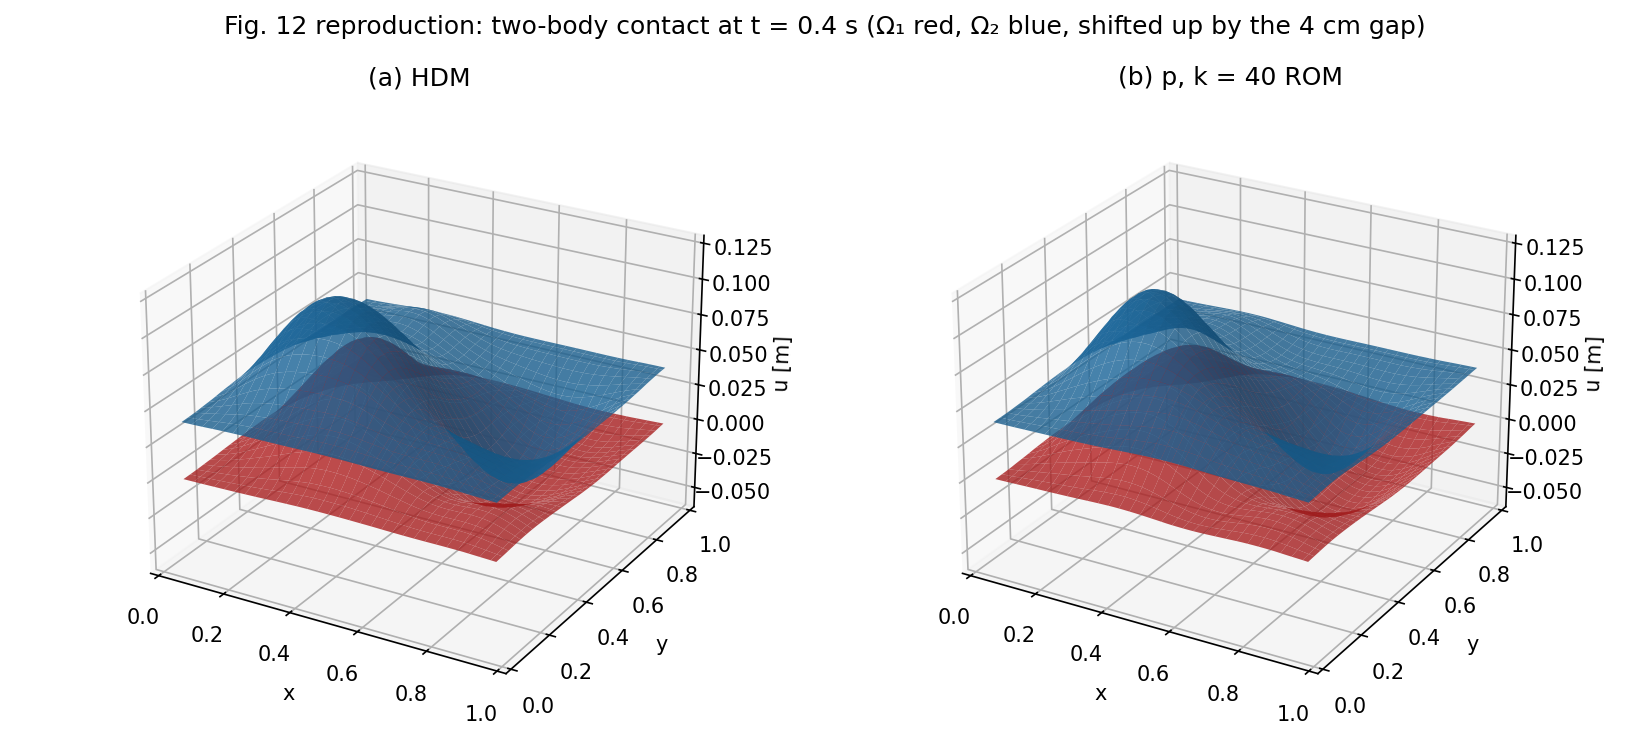
\includegraphics[width=0.95\linewidth]{figures/ch14r/bl_two3d.png}
\caption{Both plates at $t=0.4$~s: full model (left) and the $p=p_\lambda=40$ ROM (right); $\Omega_1$ red, $\Omega_2$ blue (shifted up by the gap so that touching surfaces coincide). Plot of the reproduction report.}\label{fig:vf-bl-two3d}
\end{figure}

\emph{Down-sampling.} \Cref{tab:vf-bl-down} and \Cref{fig:vf-bl-down} give the error against the percentage of snapshots kept (25 snapshots is $1.25\,\%$). The error is flat down to about $10\,\%$ kept ($p=40$: $0.7$--$1.6\,\%$) and rises sharply at $5\,\%$ or less, as in the publication; its $52.8\,\%$ at 25 snapshots is not matched (here $13.6\,\%$). The $p=20$ curve is erratic and non-monotone, which points to local minima of the NMF and rank limits and not to the number of snapshots.

\begin{table}[tbp]
\centering\footnotesize
\caption{Two plates: error (\%) against the percentage of snapshots kept.}\label{tab:vf-bl-down}
\begin{tabular}{@{}lrrrrrrr@{}}
\toprule
\% kept & 100 & 50 & 25 & 10 & 5 & 2.5 & 1.25\\
\midrule
$p=p_\lambda=20$ & 1.84 & 10.3 & 2.83 & 4.23 & 6.54 & 3.64 & 15.0\\
$p=p_\lambda=40$ & 1.36 & 1.63 & 0.70 & 0.67 & 4.28 & 2.51 & 13.6\\
$p=p_\lambda=100$ & 0.040 & 0.042 & 0.099 & 0.50 & 1.21 & 2.59 & 13.6\\
\bottomrule
\end{tabular}
\end{table}

\begin{figure}[tbp]
\centering
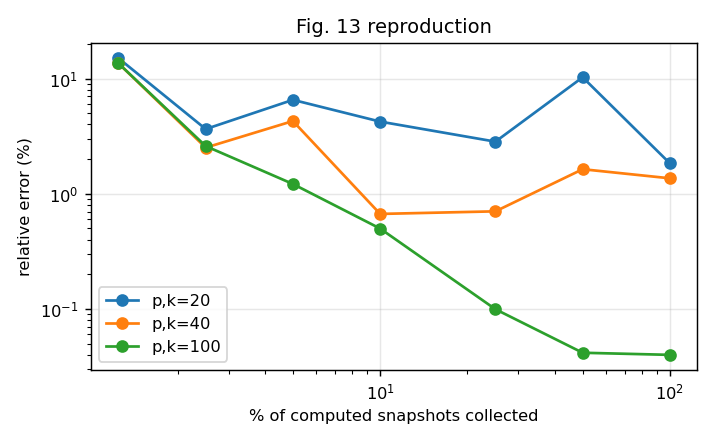
\includegraphics[width=0.7\linewidth]{figures/ch14r/bl_down.png}
\caption{Two plates: error against the percentage of snapshots kept. Plot of the reproduction report.}\label{fig:vf-bl-down}
\end{figure}

\subsection*{Speed-ups}

\Cref{tab:vf-bl-speed} compares with the publication. The comparison is not one-to-one: the publication's full-order solver used MATLAB \texttt{quadprog} (interior point), here a sparse active-set solver with warm starts (membranes) or a precomputed dense complementarity matrix (plates) is used, much faster per solve; and the ROM cost is not strictly size-independent (a dense Cholesky of the reduced matrix at every step). The robust conclusion is the trend: ROM cost is independent of $N$ while full-order cost grows at least linearly, so the speed-up grows with mesh size.

\begin{table}[tbp]
\centering\footnotesize
\caption{Speed-up against the publication's Table~I.}\label{tab:vf-bl-speed}
\begin{tabularx}{\linewidth}{@{}>{\raggedright\arraybackslash}p{2.6cm} >{\raggedright\arraybackslash}X >{\raggedright\arraybackslash}X@{}}
\toprule
Problem & Publication (full-order size, ROM size, speed-up) & This work\\
\midrule
Static obstacle & 40\,000; $p=p_\lambda=20$; 865 & 39\,601; 20/20; 1256 (full 3.72 s sparse PDAS, ROM 3.0 ms)\\
Dynamic obstacle & 40\,000; 100; 302 & 1521; 100; 14.7 measured (3.59 s, 0.245 s); about 490 extrapolated to 39\,601 dofs (119 s per run), not measured\\
Two-body & 20\,000; 40; 2229 & 3174; 40; 13.5\\
\bottomrule
\end{tabularx}
\end{table}

\subsection*{Comparison with the publication}

\begin{table}[tbp]
\centering\footnotesize
\caption{Outcome of the reproduction of \citet{balajewicz2016contact}.}\label{tab:vf-bl-cmp}
\begin{tabularx}{\linewidth}{@{}>{\raggedright\arraybackslash}p{4.3cm} >{\raggedright\arraybackslash}X >{\raggedright\arraybackslash}p{2.5cm}@{}}
\toprule
Claim & This work & Outcome\\
\midrule
Greedy beats random sampling; $p\approx10$ equals random $p=20$ (static) & $124\times$ below the random median; yes & reproduced\\
$\alpha_1$-only indicator best & identical sequences (static); $\alpha_1$-only and all-three best by a small margin (dynamic) & not reproduced\\
More than $100\times$ error drop in 10 iterations (dynamic) & $127$--$288\times$ & reproduced\\
NMF dual tracks the full model, SVD dual does not & $0.06$--$0.08\,\%$ against $\sim300\,\%$ & reproduced\\
Two plates: $p=p_\lambda=40$ tracks the full model & $1.36\,\%$ (Mindlin, 3174 dofs) & reproduced, smaller mesh\\
Insensitive to down-sampling down to about $10\,\%$ & flat to $10\,\%$, rises at $\le5\,\%$; $52.8\,\%$ at 25 snapshots not matched ($13.6\,\%$) & partly\\
Speed-ups 865, 302, 2229 & 1256, 14.7, 13.5 (different solver, smaller meshes) & not comparable\\
\bottomrule
\end{tabularx}
\end{table}

\subsection*{What was not reproduced, and why}

The static case is at the publication's size, but the dynamic and two-body cases are smaller (running the dynamic cases at the publication's size needs roughly 100 times the compute used). The plates are Mindlin elements with three degrees of freedom per node, where the publication has a Kirchhoff plate with one: linear deflection and frequency agree with Kirchhoff theory to better than $0.5\,\%$, but the contact response will differ in detail, and the publication gives no numbers beyond the $\pm0.2$~m range of its Fig.~11 to compare. The membrane discretisation is not specified beyond ``$200\times200$ elements''. The first greedy sample, the NMF algorithm and iteration count, the stopping parameter and the sign convention are unspecified and were chosen here. The oracle curve of the publication is the lowest, and the author's oracle (greedy on the true maximum error) is not, since its definition is open. Multiplier accuracy is weaker than displacement accuracy (static worst case $52\,\%$ force error, active-set overlap $0.69$) and the full-space penetration of the NMF ROM is non-zero, a point the publication does not report. Each configuration is a single run, wall-clock numbers come from a shared 12-core machine, and the full-size dynamic and 20\,000-degree-of-freedom plate cases were not run.

Four things were added or are recommended for the packages as a result: a scalar Laplace element and a sparse, non-condensed unilateral solver in \fea{} (the condensed route is fine to roughly 3000 constraints, an estimate and not a measured limit, and needs about 12.5~GB at 39\,601); BDF2 or Newmark in \texttt{solve\_contact\_dynamics} (the first-order scheme has about 28 times the BDF2 error at $\Delta t=0.005$ and about 60 times at $0.0025$, one free-membrane test); a \texttt{ContactROM.solve\_dynamic} with trajectory snapshots and the greedy growth schedule in \rom{}; and a cached pseudo-inverse in the indicator so that $\alpha_2,\alpha_3$ are usable at scale.
